\documentclass[12pt]{article}
\usepackage{amsmath,amssymb,amsfonts}
\usepackage{graphicx}
\usepackage{hyperref}
\usepackage{color}
\usepackage{tikz}
\usetikzlibrary{shapes,arrows}
\usepackage[margin=2cm]{geometry}

\title{ECSE 426 - Microprocessor Systems\\Lab Report 1: Analog Data Acquisition, Filtering, and
Digital I/O}
\author{Harley Wiltzer (260690006)\\Matthew Lesko}
\date{February 19, 2018}

\definecolor{dblue}{rgb}{0.4,0.4,0.8}

\hypersetup {
	colorlinks=true,
	linkcolor=dblue
}

\tikzstyle{decision} = [diamond, draw, fill=blue!20, text badly centered, text width=2cm, node
distance=3cm]
\tikzstyle{block} = [rectangle, draw, fill=blue!20, text centered, rounded corners, minimum
height=4em, text width=3cm, node distance=5cm]
\tikzstyle{goal} = [rectangle, draw, fill=yellow!20, text centered, rounded corners, minimum
height=4em, text width=3cm, node distance=5cm]
\tikzstyle{line} = [draw, -latex']
\tikzstyle{cloud} = [draw, ellipse, fill=red!20, node distance=7cm, text centered, text width=2cm]

\begin{document}
\maketitle
\tableofcontents
\listoffigures
\listoftables
\section{Implementation}
The design of the voltmeter was fairly complex and was composed of several modules.
These modules included the \hyperref[userinput]{user input module} for processing user input via the
push button, the \hyperref[dataaq]{data
acquisition module} for digitizing analog data on the board, the \hyperref[dataproc]{data processing
module} for filtering
the data and associating meaning to its digital values, and the output module for displaying the
data to the user. This section will be divided into several subsections, each corresponding to a
module, in order to organize the design decisions that were made.\\\\
Since all of these modules needed to work together, they had to be synchronized
appropriately, and this was achieved with the \texttt{SysTick} timer. The \texttt{SysTick} timer
invokes interrupts at a chosen frequency, and the interrupt handler was used to coordinate all of
the modules. Since the configuration parameters of the \texttt{SysTick} timer were heavily
influenced by the modules described above, they will be explained independently in the sections
following where the design decisions were made.
\subsection{The User Input Module}\label{userinput}
One of the requirements of the voltmeter was to provide three display modes to the user: a display
of the RMS voltage, and a display for each of minimum and maximum voltage updated within the past
ten seconds. As such, there was a need for user input to switch between these display modes. This
was achieved with the user button on the STM32F407 board, which allowed the user to cycle through
each of the display modes by pressing the button.\\\\
The first challenge dealt with how to process the button presses. There were two main options:
polling for button presses and handling interrupts. Since polling the button at every iteration in a
loop seemed inefficient, the interrupt method was chosen. Therefore, an NVIC interrupt was
configured at priority 0 for \texttt{EXTI0}. However, even with the interrupts set up, there was
still a major challenge to correctly process the button presses, as one button press often caused
several interrupts. This could have been do to button bouncing, or possibly the fact that a what
seems like a short \textit{click} to a human actually goes over several clock cycles of the
processor. To prevent this from occuring, it was decided to enforce a time delay between consecutive
button press handling routines, and this was achieved using the \texttt{SysTick} timer. The process
is shown in \hyperref[buttonflow]{Figure 1}.\\\\
\begin{figure}\label{buttonflow}
	\caption{Debouncing button presses}
	\begin{center}
		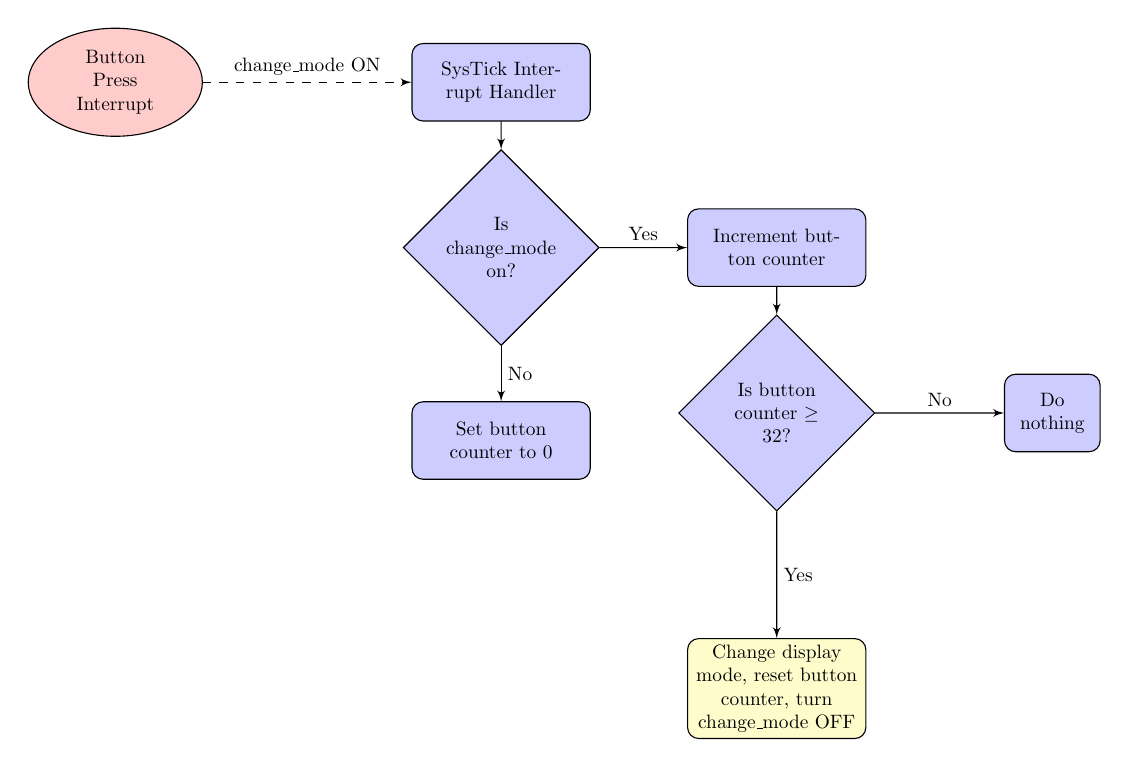
\begin{tikzpicture}[node distance = 2cm, auto, scale=0.7, transform shape]
			\node [block] (tick) {SysTick Interrupt Handler};
			\node [cloud,left of=tick] (exti0) {Button Press Interrupt};
			\node [decision, below of=tick] (ifchange) {Is change\_mode on?};
			\node [block, below of=ifchange, node distance=3.5cm] (zerobc) {Set button counter to 0};
			\node [block, right of=ifchange, node distance=5cm] (incbc) {Increment button counter};
			\node [decision, below of=incbc] (ifcount) {Is button counter $\geq$ 32?};
			\node [block, right of=ifcount, text width=1.5cm] (wait) {Do nothing};
			\node [goal, below of=ifcount] (button) {Change display mode, reset button counter, turn
			change\_mode OFF};
			\path [line, dashed] (exti0) -- node {change\_mode ON} (tick);
			\path [line] (tick) -- (ifchange);
			\path [line] (ifchange) -- node {No} (zerobc);
			\path [line] (ifchange) -- node {Yes} (incbc);
			\path [line] (incbc) -- (ifcount);
			\path [line] (ifcount) -- node {No} (wait);
			\path [line] (ifcount) -- node {Yes} (button);
		\end{tikzpicture}
	\end{center}
\end{figure}
\textit{In brevarium}, the \texttt{EXTI0\_IRQHandler()} function (invoked by the button press
interrupt) asserts a \texttt{change\_mode} signal, and when the \texttt{SysTick\_Handler()} function
(invoked by \texttt{SysTick} interrupt) sees that, it waits for 32 consecutive \texttt{SysTick}
interrupts before taking action. The number 32 was achieved via trial and error, as it was unknown
exactly how long an average human button press lasts. That being said, this number was chosen at a
\texttt{SysTick} frequency of 200Hz, so a delay of 160ms was imposed.

\subsection{The Data Acquisition Module}\label{dataaq}
The data acquisition module was responsible for gathering analog data and digitizing it so it could
be processed. Firstly, however, it was helpful to set up a digital to analog converter (DAC) in
order to test the performance of the analog to digital converter (ADC). Setting up the DAC was
fairly straightforward, and most of the work was carried out by the HAL Cube software. The DAC was
configured on channel 1, and it wrote to pin PA4 on the board. Furthermore, its resolution had to be
chosen. Since the performance of the voltmeter ultimately depended on the resolution of the ADC, the
resolution of the DAC was chosen to be the same as that of the ADC, which was 8 bits, right aligned.
This decision will be explained when discussing the ADC parameters below. Finally, the DAC needed to
output some analog voltage. A value was chosen arbitrarily and passed to the DAC via the
\texttt{HAL\_DAC\_SetValue()} driver function, and the conversion was instantiated via
\texttt{HAL\_DAC\_Start()}. This starts a conversion in polling mode, which was deemed appropriate
for the purposes of this experiment as the conversion would only occur once.\\\\
Setting up the ADC was considerably more complicated. Again, the basic initialization was done by
the HAL Cube software, and the ADC1 unit was set up on channel 1. Single conversion mode was chosen,
as it was required for one conversion to occur at a given frequency. Once again, the resolution had
to be determined. Since it was known that the displayed voltages would be shown with two decimal
places of precision, the user could only see voltages in increments of $0.01$V. 
\begin{table}[h]\label{adcres}
	\caption{Accuracy of ADC by resolution}
	\begin{center}
		\begin{tabular}{|c|c|}
			\hline
			Resolution (bits) & Voltage difference between consecutive digital values (V)\\\hline
			6 & 0.047\\\hline
			8 & 0.012\\\hline
			10 & 0.003\\\hline
			12 & 4.89e-4\\\hline
		\end{tabular}
	\end{center}
\end{table}
The accuracy of the ADC by its resolution is shown in \hyperref[adcres]{Table 1}. The accuracy is
defined here as the change in voltage when increasing the digital reading by 1. Since the voltage
range of the ADC is 3V, the accuracies were calculated according to
\begin{equation}
	A = \frac{3}{2^{R}}
\end{equation}
were $A$ is the accuracy (rightmost column) and $R$ is the resolution (leftmost column). Clearly, a
resolution of 6 bits is not a great choice, as it cannot resolve voltages within 0.047V from each
other. Since the display of the voltmeter allowed two decimal places, this accuracy is insufficient.
With a resolution of 10 bits, however, the accuracy is relatively high. At an accuracy of 0.003V,
the display would only change after a change of 4 in the digital reading of the ADC. The 8 bit
resolution could resolve voltages that are 0.012V apart which is very close to the accuracy on the
display. Ultimately, the 8 bit and 10 bit resolutions were the main contenders, because the 8 bit
resolution is slightly worse than that of the display, and the 10 bit resolution is much stronger
than that of the display. In the end, the 8 bit resolution was chosen as it was deemed strong enough
for the purposes of this experiment, it would cause lower power consumption, and it matched one of
the possible resolutions of the DAC which made the code simpler.\\\\
Next, the conversion mode of the ADC had to be chosen. Polling mode was not considered a viable
option, since ADC conversions would happen frequently and thus polling would waste a considerable
portion of the CPU's cycles. Although DMA was a very good alternative, the developers did not have
time to do the requisite research. Therefore, interrupt mode was selected. Despite the conversion
mode, however, the frequency of ADC conversions remained to be implemented. A sample rate of 50Hz
was required, so the \texttt{SysTick} interrupts were used to time the ADC conversions. Since the
\texttt{SysTick} interrupts were occuring at 200Hz (see the Output subsection below), it was
required to implement a prescaler in the \texttt{SysTick\_Handler()} function in order to sample at
50Hz.
\begin{figure}[h]\label{adcflow}
	\caption{Flow of ADC processing}
	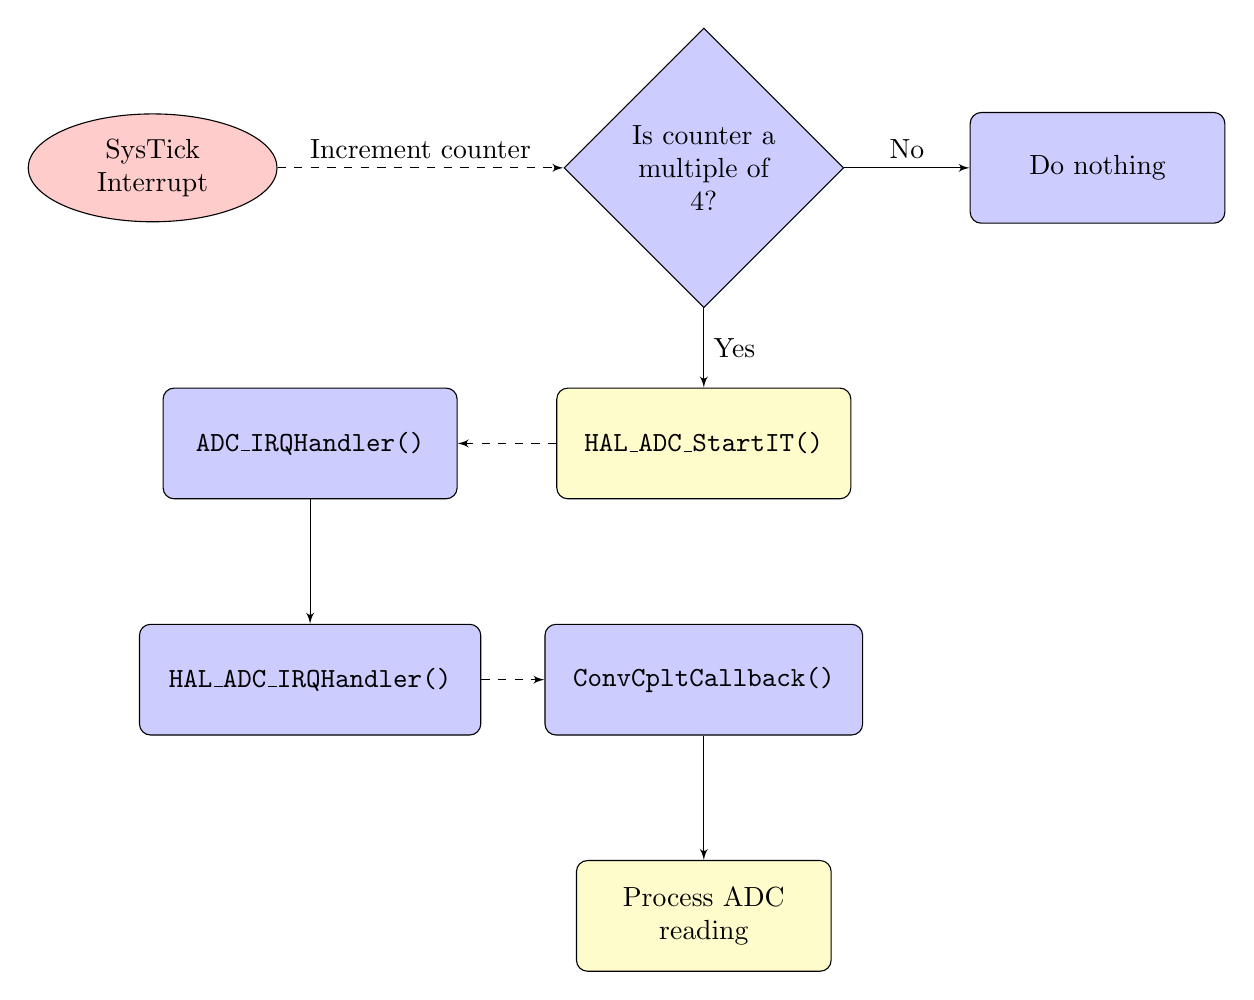
\begin{tikzpicture}[node distance=2cm, auto]
		\node [cloud, node distance=7cm] (systick) {SysTick Interrupt};
		\node [decision, right of=systick,node distance=7cm] (ifcount) {Is counter a multiple of 4?};
		\node [block, right of=ifcount] (nothing) {Do nothing};
		\node [goal, below of=ifcount, text width=3.5cm, node distance=3.5cm] (startadc) {\texttt{HAL\_ADC\_StartIT()}};
		\node [block, left of=startadc, text width=3.5cm] (irqhandler) {\texttt{ADC\_IRQHandler()}};
		\node [block, below of=irqhandler, text width=4.1cm, node distance=3cm] (haladc)
		{\texttt{HAL\_ADC\_IRQHandler()}};
		\node [block, right of=haladc, text width=3.8cm] (conv) {\texttt{ConvCpltCallback()}};
		\node [goal, below of=conv, node distance=3cm] (processadc) {Process ADC reading};
		\path [line, dashed] (systick) -- node {Increment counter} (ifcount);
		\path [line] (ifcount) -- node {No} (nothing);
		\path [line] (ifcount) -- node {Yes} (startadc);
		\path [line, dashed] (startadc) -- (irqhandler);
		\path [line] (irqhandler) -- (haladc);
		\path [line, dashed] (haladc) -- (conv);
		\path [line] (conv) -- (processadc);
	\end{tikzpicture}
\end{figure}
The process of handling ADC conversions is shown in \hyperref[adcflow]{Figure 2}. The
\texttt{SysTick\_Handler()} maintains a \texttt{counter} and increments it at every \texttt{SysTick}
interrupt, that is to say, at 200Hz. Since ADC conversions were to be taken at 50Hz, they had to be
triggered at a rate four times less frequent than \texttt{SysTick}. Thus, the
\texttt{HAL\_ADC\_StartIT()} function was called on every fourth \texttt{SysTick} interrupt to start
ADC conversions at 50Hz. This was accomplished by starting the ADC conversion when the
\texttt{counter} variable was a multiple of 4.

\subsection{The Data Processing Module}\label{dataproc}
\end{document}
